\documentclass[tikz,border=3pt]{standalone}
\usetikzlibrary{arrows.meta,calc}
\begin{document}
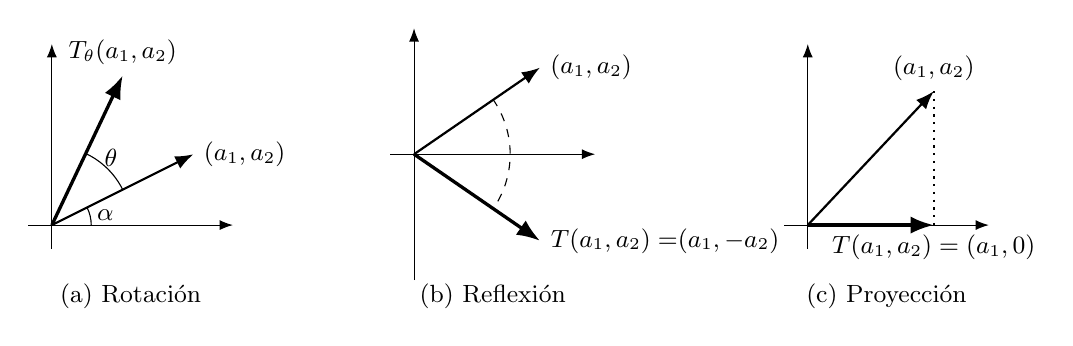
\begin{tikzpicture}[>=Latex, font=\small]
  % --- panel (a): rotacion ---
  \begin{scope}
    \draw[->] (-0.3,0) -- (2.3,0);
    \draw[->] (0,-0.3) -- (0,2.3);
    \draw[->, thick] (0,0) -- (1.8,0.9) node[right] {$(a_1,a_2)$};
    \draw[->, very thick] (0,0) -- (0.9,1.9) node[above] {$T_\theta(a_1,a_2)$};
    \draw (0.5,0) arc (0:26.5:0.5);
    \node at (0.68,0.13) {$\alpha$};
    \draw (0.9,0.45) arc (26.5:64.5:1.0);
    \node at (0.75,0.85) {$\theta$};
    \node at (1.0,-0.9) {(a) Rotación};
  \end{scope}

  % --- panel (b): reflexion ---
  \begin{scope}[shift={(4.6,0.9)}]
    \draw[->] (-0.3,0) -- (2.3,0);
    \draw[->] (0,-1.6) -- (0,1.6);
    \draw[->, thick] (0,0) -- (1.6,1.1) node[right] {$(a_1,a_2)$};
    \draw[->, very thick] (0,0) -- (1.6,-1.1) node[right] {$T(a_1,a_2)=$\\$(a_1,-a_2)$};
    \draw[dashed] (1.0,0.7) arc (35:-35:1.22);
    \node at (1.0,-1.8) {(b) Reflexión};
  \end{scope}

  % --- panel (c): proyeccion ---
  \begin{scope}[shift={(9.6,0)}]
    \draw[->] (-0.3,0) -- (2.3,0);
    \draw[->] (0,-0.3) -- (0,2.3);
    \draw[->, thick] (0,0) -- (1.6,1.7) node[above] {$(a_1,a_2)$};
    \draw[dotted, thick] (1.6,1.7) -- (1.6,0);
    \draw[->, very thick] (0,0) -- (1.6,0);
    \node[below] at (1.6,0) {$T(a_1,a_2)=(a_1,0)$};
    \node at (1.0,-0.9) {(c) Proyección};
  \end{scope}
\end{tikzpicture}
\end{document}
